\documentclass[UTF8,a4paper]{article}% 文档格式
\usepackage{graphicx}
\usepackage{physics}
\usepackage{ctex}
\usepackage{times}% 英文使用Times New Roman
\usepackage[left=1cm,right=1cm,top=1.80cm,bottom=1.8cm]{geometry}
\usepackage{fancyhdr}
\pagestyle{fancy}
\usepackage{multirow}
\usepackage{siunitx}
\usepackage{float}

\title{\textbf{基础物理实验报告\\电磁感应}}
\author{杨哲涵~~~工物22班~~~2022011105}
\date{2023年11月2日}
\begin{document}
\maketitle
\lhead{2023年基础物理学实验A2}
\chead{}
\rhead{42a}
\lfoot{}
\cfoot{\thepage}
\rfoot{}
\section*{摘要}
处于变化磁通量之中的导体,会产生电动势,这种现象被称为电磁感应.本实验利用两个线圈构成的耦合线圈系统探究自感与互感的相关结论,得到了关于等效阻抗与反射物理量之间的一系列关系.特别地,对铝芯插入前后的分析展示了涡流探伤的原理.
\section{实验原理与仪器}
\paragraph{正弦稳态电路原理}
正弦稳态电路中,运用相量法可以方便地分析求解电路响应.即采用$\dot{I}=Ie^{j\phi_i},\dot{U}=Ue^{j\phi_u}$这样的形式表示电流与电压.其中$I,U$为有效值,频率需要另外告知.

此外,根据电磁学知识,电感元件的伏安关系为$u=L\dv{i}{t}$,若采用相量形式表示,有$\dot{U}=j\omega L\dot{I}$.如果记感抗$X_L=j\omega L$,阻抗$Z=R+jX$.那么电阻,电容,电感的响应可以被统一地考虑了.

由于实验中只能测量有效值,我们可以针对$U,I$列出关系:
$$U^2=\dot{U}^*\dot{U}=(IR)^2+(IX)^2$$
这也给出了阻抗三角形的结论$Z=\sqrt{R^2+X^2}$.

之前在直流电路中的KVL,KCL等定律以及相应的分析方法都可以用来分析正弦稳态电路,只要相关的量都是用相量形式表达的.

另外,我们会好奇关于功率的结论,考虑一般的$\dot{U}=\dot{I}(R+jX)$,可以发现$\dot{U}\dot{I}^*=RI^2+jXI^2$.若对其积分后取平均值,可以发现只有$RI^2$仍然保留,$XI^2$消失了.意味着系统的平均功率仅由电阻决定.这背后的原因是电阻会消耗能量,电容与电感只会将电能储存与释放.因此$\Re[\dot{U}\dot{I}^*]$被记为有功功率,代表电路实际消耗能量的速率.
\paragraph{实验仪器}
实验用到了信号发生器,电缆(连接线),手持万用表,数字电表,面包板,定值电阻与电阻板,以及铝棒和线圈(1和2).
\section{实验内容}
\subsection{测量无芯线圈和铝芯线圈内阻和电感}
\begin{table}[H]
    \centering
    \caption{a-d部分数据记录及计算}
    \label{tb:a-d}
    \begin{tabular}{l|llllllllllll}
        \hline
             & $R^\prime(\unit{\ohm})$ & $V_A(\unit{\volt})$ & $V(\unit{\volt})$ & $V_{R^\prime}(\unit{\volt})$ & $V_o(\unit{\volt})$ & $I(\unit{\A})$ & $Z(\unit{\ohm})$ & $R(\unit{\ohm})$ & $X(\unit{\ohm})$ & $L(\unit{\mH})$ & $\omega M  $ & $M(\unit{\mH})$ \\
        \hline
        1无铝芯 & 560                     & 6.777               & 4.569             & 4.593                        & 3.898               & 0.008          & 557.06           & 52.52            & 554.58           & 88.26           & 475.26       & 75.640          \\
        1有铝芯 & 460                     & 6.714               & 4.359             & 4.356                        & 3.075               & 0.009          & 460.32           & 86.09            & 452.20           & 71.96           & 324.72       & 51.682          \\
        2无铝芯 & 630                     & 6.813               & 4.621             & 4.620                        & 3.481               & 0.007          & 630.16           & 54.86            & 627.77           & 99.91           & 474.68       & 75.548          \\
        2有铝芯 & 410                     & 6.675               & 4.133             & 4.085                        & 3.235               & 0.010          & 414.82           & 132.51           & 393.08           & 62.56           & 324.69       & 51.676          \\
        \hline
    \end{tabular}
\end{table}
可知对于线圈1和2,有:
\begin{align*}
     & R_1=52.52\unit{\ohm}\qq{}L_1=88.26\unit{\mH}     \\
     & R_2=54.86\unit{\ohm}\qq{}L_2=99.91\unit{\mH}     \\
     & R_1^*=86.09\unit{\ohm}\qq{}L_1^*=71.96\unit{\mH} \\
     & R_2^*=132.5\unit{\ohm}\qq{}L_2^*=62.56\unit{\mH}
\end{align*}

\subsection{互感和耦合常数}
针对线圈1在无铝芯的情况下,将$R^\prime$固定为300$\unit{\ohm}$,有表\ref{tb:g-n}展示的测量记录与计算结果:

\begin{table}[H]
    \centering
    \caption{g-n部分数据记录及计算}
    \label{tb:g-n}
    \begin{tabular}{lllllllllllll}
        \hline
        $R_L(\unit{\ohm})$ & $R^\prime(\unit{\ohm})$ & $V_A(\unit{\volt})$ & $V(\unit{\volt})$ & $V_{R^\prime}(\unit{\volt})$ & $V_{RL}(\unit{\volt})$ & $I_p(\unit{\A})$ & $Z_p(\unit{\ohm})$ & $R_{PE}(\unit{\ohm})$ & $X_{PE}(\unit{\ohm})$ & $X_R(\unit{\ohm})$ & $I_s(\unit{\A})$ & $R_R(\unit{\ohm})$ \\
        \hline
        100.00             & 300.00                  & 6.48                & 3.37              & 4.02                         & 0.99                   & 0.01             & 251.64             & 133.42                & 213.36                & 340.14             & 0.010            & 83.97              \\
        200.00             & 300.00                  & 6.53                & 3.67              & 3.67                         & 1.72                   & 0.01             & 299.89             & 175.43                & 243.22                & 309.28             & 0.009            & 125.66             \\
        300.00             & 300.00                  & 6.58                & 3.95              & 3.42                         & 2.26                   & 0.01             & 346.82             & 204.62                & 280.02                & 274.89             & 0.008            & 155.51             \\
        400.00             & 300.00                  & 6.62                & 4.19              & 3.25                         & 2.66                   & 0.01             & 386.58             & 221.97                & 316.50                & 236.75             & 0.007            & 171.67             \\
        500.00             & 300.00                  & 6.64                & 4.38              & 3.14                         & 2.97                   & 0.01             & 419.16             & 229.83                & 350.53                & 202.69             & 0.006            & 179.29             \\
        600.00             & 300.00                  & 6.66                & 4.54              & 3.06                         & 3.22                   & 0.01             & 445.42             & 231.21                & 380.71                & 173.22             & 0.005            & 180.84             \\
        700.00             & 300.00                  & 6.68                & 4.67              & 3.01                         & 3.41                   & 0.01             & 465.99             & 228.55                & 406.09                & 147.82             & 0.005            & 177.88             \\
        800.00             & 300.00                  & 6.70                & 4.78              & 2.97                         & 3.56                   & 0.01             & 482.09             & 223.33                & 427.24                & 126.55             & 0.004            & 172.47             \\
        900.00             & 300.00                  & 6.71                & 4.87              & 2.95                         & 3.69                   & 0.01             & 494.88             & 216.72                & 444.90                & 108.99             & 0.004            & 165.91             \\
        1000.00            & 300.00                  & 6.71                & 4.94              & 2.94                         & 3.80                   & 0.01             & 505.10             & 209.73                & 459.51                & 94.43              & 0.004            & 158.81             \\ \hline
    \end{tabular}
\end{table}

可以使用$\omega MI_p=I_sZ_s$的展开为依据做拟合,具体为:
$$\omega^2M^2\frac{I_p^2}{I_s^2}-X_s^2=(R_s+R_L)^2$$
因此如果以$\frac{I_p^2}{I_s^2}$作为$x$,$(R_s+R_L)^2$作为$y$,其中$R_s$带入线圈2在无铝芯下的电阻,那么直线拟合的截距为$-X_s^2$,斜率为$\omega^2M^2$.

拟合中间计算结果如表\ref{tb:linest}所示,其关系式展示在图\ref{fg:linest}之中.
\begin{table}[H]
    \centering
    \caption{互感与感抗的直线拟合}
    \label{tb:linest}
    \begin{tabular}{l|llllllllll}
        \hline
        $x=(I_p/I_s)^2$ & 1.8441 & 2.0282 & 2.2819 & 2.6495 & 3.0948 & 3.6212 & 4.2436 & 4.9566 & 5.7553 & 6.6423  \\
        $y=(R_s+R_L)^2$ & 23980  & 64951  & 125923 & 206894 & 307865 & 428837 & 569808 & 730779 & 911751 & 1112722 \\ \hline
    \end{tabular}
\end{table}
可以得到$M=75.808\unit{\mH}\qq{}X_s=627.499\unit{\ohm}$.
\begin{figure}[H]
    \centering
    \begin{minipage}[t]{0.45\linewidth}
        \centering
        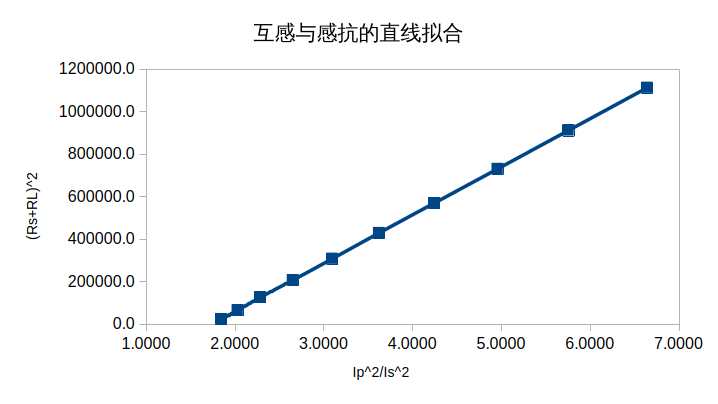
\includegraphics[width=1.0\linewidth]{linest.png}
        \caption{互感与感抗的直线拟合}
        \label{fg:linest}
    \end{minipage}
    \begin{minipage}[t]{0.45\linewidth}
        \centering
        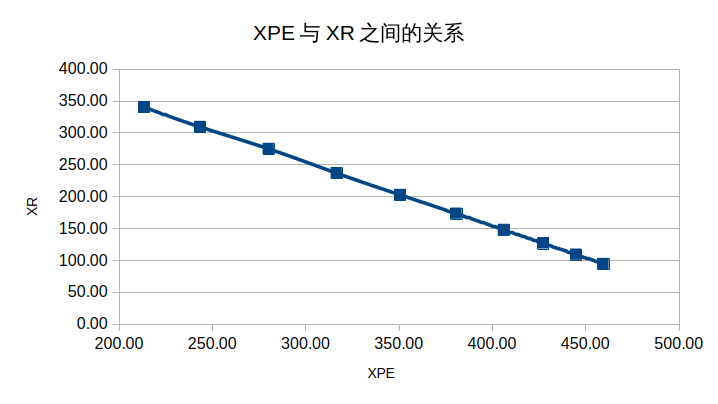
\includegraphics[width=1.0\linewidth]{xpe-xr.png}
        \caption{$X_{PE}$随$X_R$的变化}
        \label{fg:xpe-xr}
    \end{minipage}
    \begin{minipage}[t]{0.45\linewidth}
        \centering
        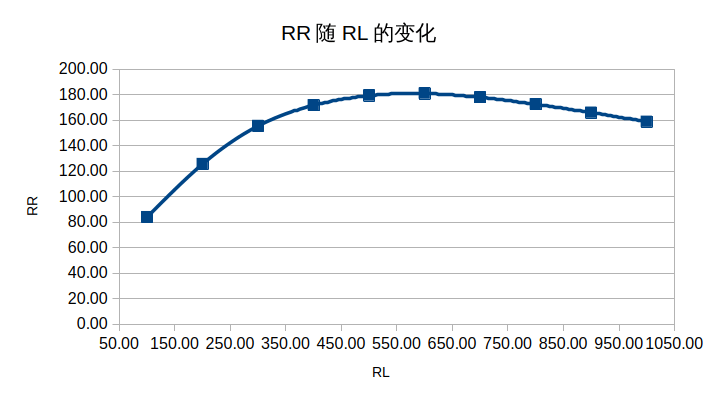
\includegraphics[width=1.0\linewidth]{rr-rl.png}
        \caption{$R_R$随$R_L$的变化}
        \label{fg:rr-rl}
    \end{minipage}
    \begin{minipage}[t]{0.45\linewidth}
        \centering
        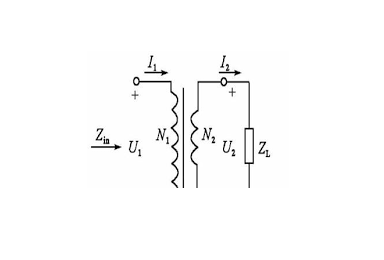
\includegraphics[width=1.0\linewidth]{mutual-induction.png}
        \caption{异名端互感}
        \label{fg:mutual-induction}
    \end{minipage}
\end{figure}

\subsection{初级线圈的等效阻抗和次级线圈的若干反射物理量之间的关系}
讲义给出的公式形式为$\omega MI_p=I_sZ_s$,两线圈互感的方式为非同名端互感,因此有
\begin{align*}
    \dot{U_p}                               & =(R_p+j\omega L_p)\dot{I_p}-j\omega M\dot{I_s} \qq{非同名互感} \\
    j\omega M\dot{I_p}-j\omega L_s\dot{I_s} & =\dot{I_s}(R_s+R_L) \qq{KVL}
\end{align*}

对比$\dot{U_p}=(R_{PE}+jX_{PE})\dot{I_p}$,其中需要使用$\frac{\omega^2M^2}{Z_s^2}=\frac{I_s^2}{I_p^2}$进行化简.令实部等于实部,虚部等于虚部,可以得到反射阻抗与等效阻抗之间的关系为:
\begin{align*}
    X_{PE} & =X_p-X_R \\
    R_{PE} & =R_p+R_R
\end{align*}
所要求的$R_R$与$X_R$的计算结果,已经在表\ref{tb:g-n}中列出.

此外,反射电阻
$$R_R=\frac{\omega^2M^2}{X_s^2+(R_s+R_L)^2}(R_s+R_L)$$
理论上可以得到$(R_s+R_L)=X_s$时,$R_R$最大.因此应该有$R_L=572.76\unit{\ohm}$.从图中读出的最大值在560$\unit{\ohm}$左右,符合计算的预测.
\subsection{涡流效应}
对于加入铝芯后的情况的分析,复合了铝芯的线圈所测得的阻抗实际上是等效阻抗.可以依靠反射物理量与等效阻抗的关系讨论铝芯$L_{al}$与$R_{al}$的比值.

设涡流电流为$I_{al}$,有$I^2R_R=I_{al}^2R_{al}$以及$I^2L_R=I_{al}^2L_{al}$.再由之前得到的关系,可知:
$$\frac{L_{al}}{R_{al}}=\frac{X_R}{\omega R_R}=\frac{X_p-X_{PE}}{\omega(R_{PE}-R_p)}$$
对于线圈1,结果为$\num{4.855e-4}\unit{\H/\ohm}$,线圈2的结果为$\num{4.809e-4}\unit{\H/\ohm}$.因此$L_{al}/R_{al}$的平均值约为$\num{4.832e-4}\unit{\H/\ohm}$.

对于功率的计算,始终应当按照$P=I^2R$计算有功功率.现考虑,铝芯外消耗的功率$P_0=I_s^2(R_L+R_s)+I_p^2R_p$.包括铝芯在内的消耗为$P_1=\Re[\dot{U_p}\dot{I_p}^*]$.由于$\dot{U_p}=\dot{I_p}(R_{PE}+jX_{PE})$,带入可知$P_1=I_p^2R_{PE}$.
$$\qq{因此}\Delta P=I_p^2(R_{PE}-R_p)-I_s^2(R_L+R_s)$$
得到涡流带来的功率损耗为0.0325$\unit{\W}$,相关数据列于表\ref{tb:power}.
\begin{table}[H]
    \centering
    \caption{损失功率的计算}
    \label{tb:power}
    \begin{tabular}{llllllllllll}
        \hline
        $R_L(\unit{\ohm})$ & $R^\prime(\unit{\ohm})$ & $V_A(\unit{\volt})$ & $V(\unit{\volt})$ & $V_{R^\prime}(\unit{\volt})$ & $V_{RL}(\unit{\volt})$ & $I_p(\unit{\A})$ & $Z_p(\unit{\ohm})$ & $R_{PE}(\unit{\ohm})$ & $X_{PE}(\unit{\ohm})$ & $I_s(\unit{\A})$ & $\Delta P(\unit{\W})$ \\
        1000.00            & 300.00                  & 6.66                & 4.71              & 3.30                         & 2.99                   & 0.01             & 427.31             & 155.34                & 398.07                & 0.0030           & 0.0325                \\ \hline
    \end{tabular}
\end{table}
\section{分析讨论}
\paragraph{次级线圈是否永远都是非同名端互感?}
是的.在次级线圈电流由初级线圈引起的情况下,次级线圈的电流总是落后初级线圈$\frac{\pi}{2}$,并且方向总是与初级线圈的相反,如图\ref{fg:mutual-induction}所示.由于电流方向相反,使得初级线圈处受到次级线圈的影响为$-j\omega M\dot{I_2}$.这一符号总是负的.
\paragraph{铝芯降低了互感线圈的耦合}
工程上定义$k=\frac{M}{\sqrt{L_1L_2}}$为耦合系数,耦合系数越大,代表两个线圈共用的磁通量越大,可以根据表\ref{tb:a-d}的数据计算得到,无铝芯时,$k=0.805$;有铝芯时,$k=0.770$.

可以发现,铝芯降低了两线圈耦合,这与铝芯是抗磁材料有关.
\end{document}